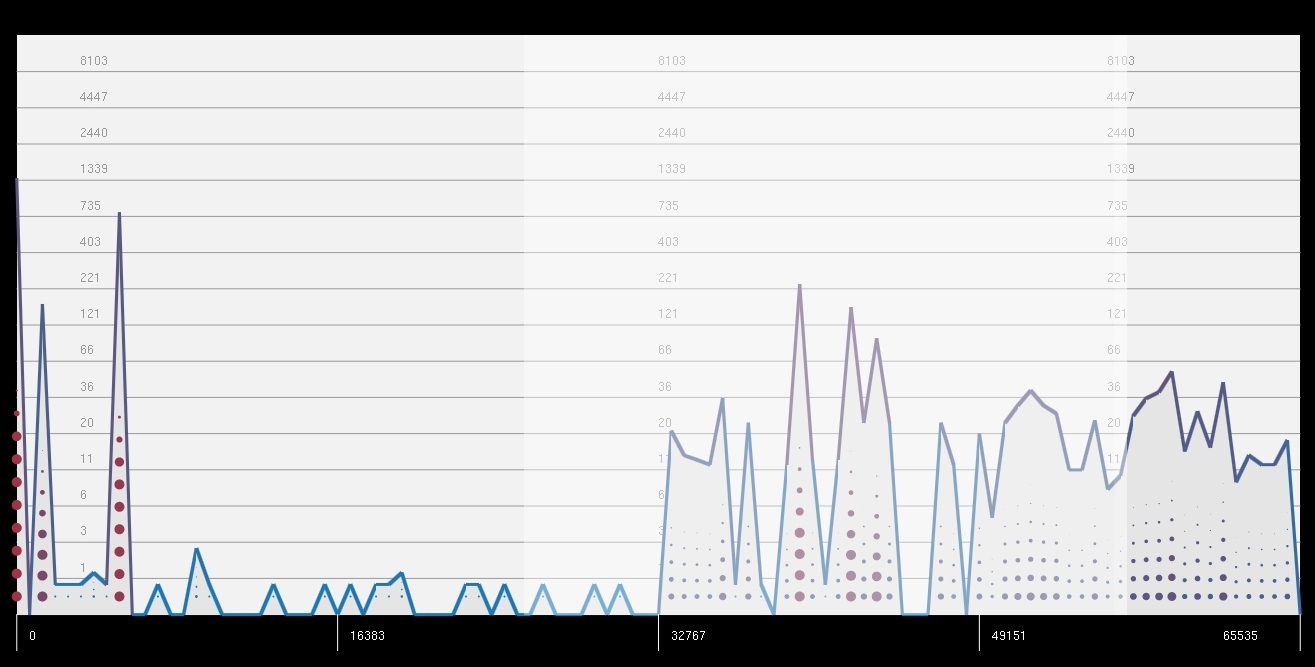
\includegraphics[width=\linewidth]{materials/distribution.jpg}

Displays a graph of the distribution of some packet attribute using its normalised value.
It improves upon existing distribution visualizations by offering a dual representation.
There is a logarithmic line graph layer useful for detecting spikes in the data and a layer of circles that indicates the actual distribution (no logarithm applied) through their area. 
Everything is colour coded to give an extra indicative of the volume of traffic (red means bigger than blue).
All these ideas have a single purpose: make the analyst understand what is going on. // maybe you can change this into something that makes more sense (combine different ideas into one visualisation...)
In this visualisation you can select a range for an attribute and the visualisation will apply a removable data filter that will only allow data in that range to get to the visualisations.
